\chapter{La synthèse~: rendement et pureté}\label{ch:g10:synthesis-yield}

L'aspirine est l'un des médicaments les plus utilisés au monde. Son
histoire commence avec l'écorce de saule, longtemps mâchée contre la
douleur et la fièvre~; au \textsc{xix}\textsuperscript{e}~siècle, on a
attribué la substance active de l'écorce à une famille de composés à
partir desquels les chimistes ont préparé l'acide salicylique. Trop
agressif pour l'estomac pour être pris à forte dose, l'acide salicylique
a été transformé en une substance plus douce, l'acide acétylsalicylique~:
l'aspirine. On la fabrique aujourd'hui à la tonne dans des réacteurs en
acier, par la même réaction qu'un laboratoire de lycée peut réaliser en
un après-midi. Fabriquer une substance n'est que la moitié du travail~:
il faut encore la séparer de tout le reste du ballon, la purifier, la
contrôler, et la peser pour voir quelle part de ce qui était possible a
réellement été obtenue.

\begin{recall}
L'\omterm{def:g10:chemical-species:extraction}{extraction}, la \omterm{def:g10:chemical-species:distillation}{distillation}, la \omterm{def:g10:chemical-species:tlc}{chromatographie sur couche mince} et le
\omterm{def:g10:chemical-species:retention-factor}{rapport frontal}~; un solide pur fond à une température nette et connue
(\cref{ch:g10:chemical-species}). Un filtre retient un solide et laisse
passer un liquide (\cref{ch:g3:separating-mixtures}). Le \omterm{def:g10:reaction-progress-table:extent}{tableau
d'avancement} donne la quantité maximale de produit à partir du \omterm{def:g10:reaction-progress-table:limiting}{réactif
limitant} (\cref{ch:g10:reaction-progress-table}).
\end{recall}

\begin{omfigure}
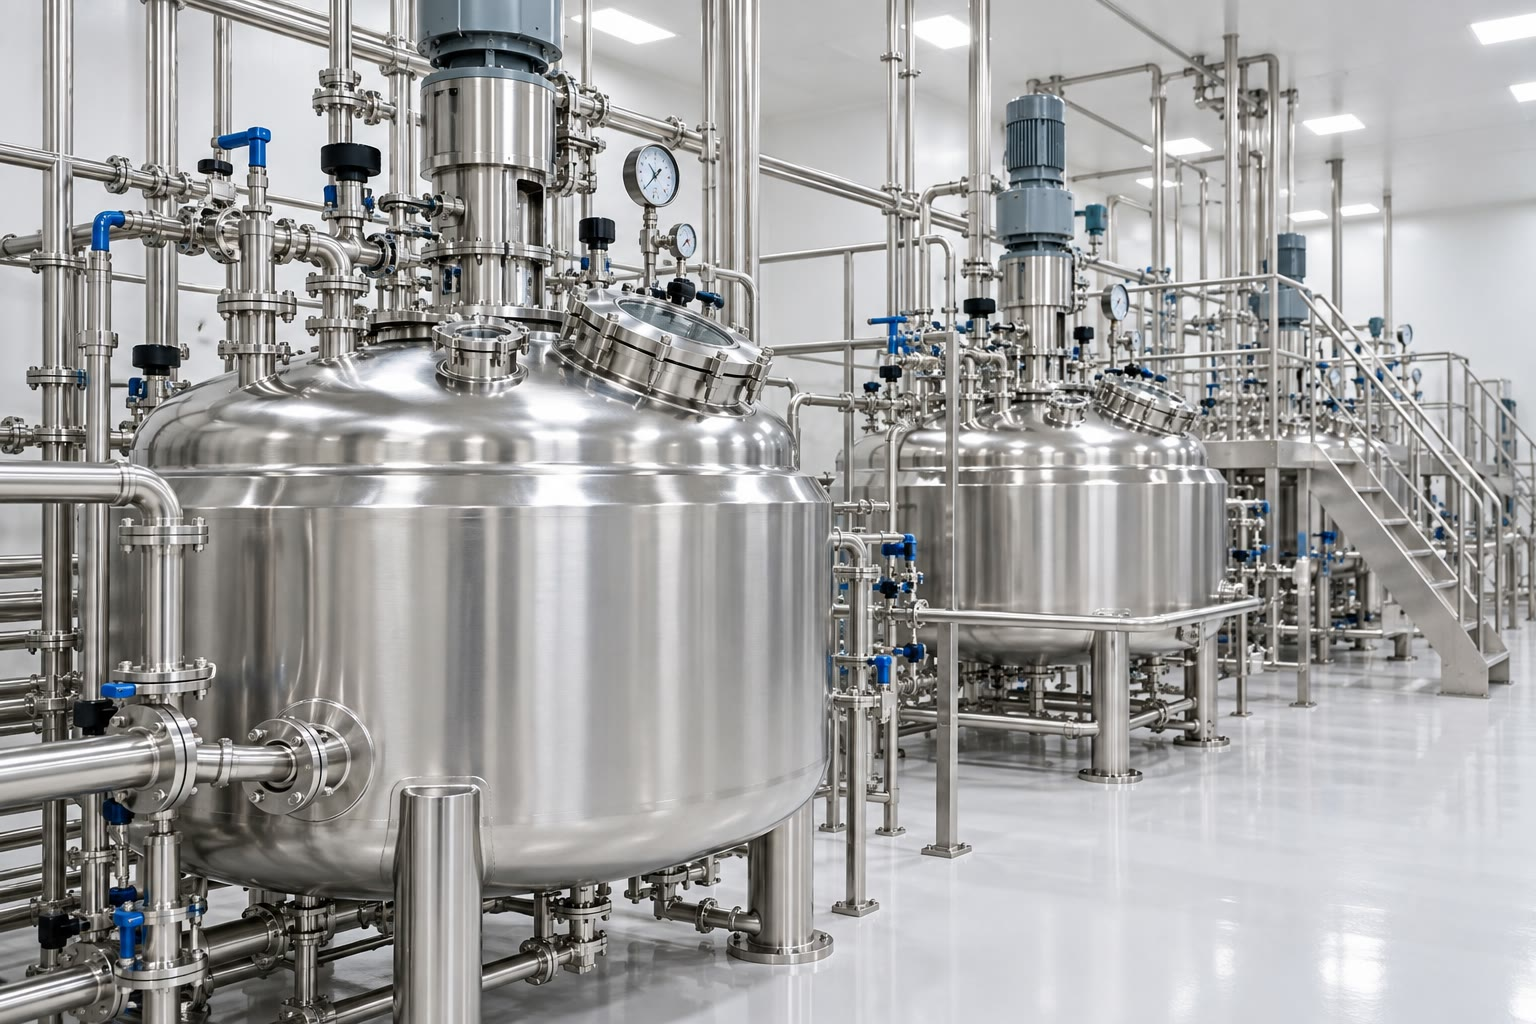
\includegraphics[width=0.55\linewidth]{images/book1/ai/g10-pharma-reactor.jpg}

{\small Des réacteurs en acier dans une usine pharmaceutique~: une
\omterm{def:g10:synthesis-yield:synthesis}{synthèse} de laboratoire, à une échelle un million de fois plus grande.}
\end{omfigure}

\section{Les étapes d'une synthèse}

\begin{definition}[Synthèse, produit brut]\label{def:g10:synthesis-yield:synthesis}
Une \emph{synthèse}\index{synthese@synthèse} est la préparation d'une \omterm{def:g6:pure-substances-and-mixtures:species}{espèce
chimique} par une ou plusieurs \omterm{def:g7:chemical-reactions:reaction}{réactions chimiques}, à partir d'autres
espèces. Le solide ou le liquide récupéré directement à partir du
\omterm{def:g6:pure-substances-and-mixtures:mixture}{mélange} réactionnel, avant toute purification, est le \emph{produit
brut}\index{produit brut}~: il contient encore des \omterm{def:g7:chemical-reactions:reactant}{réactifs}, des
sous-produits et du \omterm{def:g6:solutions-and-solubility:solute}{solvant}.
\end{definition}

\begin{method}[Organiser une synthèse]\label{met:g10:synthesis-yield:plan}
Une \omterm{def:g10:synthesis-yield:synthesis}{synthèse} se déroule en quatre étapes~:
\begin{enumerate}
  \item \textbf{Transformation}~: \omterm{def:g2:mixing-and-dissolving:mix}{mélanger} les \omterm{def:g7:chemical-reactions:reactant}{réactifs} dans les bonnes
        proportions, souvent avec l'un d'eux en excès, et chauffer si
        nécessaire.
  \item \textbf{Isolement}~: séparer le \omterm{def:g10:synthesis-yield:synthesis}{produit brut} du \omterm{def:g6:pure-substances-and-mixtures:mixture}{mélange}
        réactionnel (\omterm{def:g3:separating-mixtures:filter}{filtration}, \omterm{def:g10:chemical-species:extraction}{extraction}).
  \item \textbf{Purification}~: éliminer les impuretés du \omterm{def:g10:synthesis-yield:synthesis}{produit brut}
        (\omterm{def:g10:synthesis-yield:recrystallisation}{recristallisation} pour un solide, \omterm{def:g10:chemical-species:distillation}{distillation} pour un
        liquide).
  \item \textbf{Analyse}~: contrôler l'identité et la pureté du produit
        (température de fusion, chromatographie), puis le peser et
        calculer le \omterm{def:g10:synthesis-yield:yield}{rendement}.
\end{enumerate}
\end{method}

\begin{example}[Fabriquer de l'aspirine]\label{ex:g10:synthesis-yield:aspirin}
L'acide salicylique réagit avec l'anhydride éthanoïque (aussi appelé
anhydride acétique) pour donner l'aspirine et l'acide éthanoïque~:
\[
  \ce{C7H6O3 + C4H6O3 -> C9H8O4 + C2H4O2}
\]
\[
  \text{acide salicylique} + \text{anhydride éthanoïque} \longrightarrow
  \text{aspirine} + \text{acide éthanoïque}.
\]
L'anhydride est mis en excès, pour que tout l'acide salicylique
réagisse~; l'acide éthanoïque formé est un sous-produit.
\end{example}

\begin{omfigure}
\setchemfig{atom sep=1.7em}
\begin{tabular}{@{}c@{\enspace}c@{\enspace}c@{\enspace}c@{\enspace}c@{\enspace}c@{\enspace}c@{}}
\chemfig{*6(-=-(-COOH)=(-OH)-=)} & $+$ &
\chemfig{H_3C-C(=[2]O)-O-C(=[2]O)-CH_3} & $\longrightarrow$ &
\chemfig{*6(-=-(-COOH)=(-O-[:150]C(=[:90]O)-[:210]H_3C)-=)} & $+$ &
\chemfig{H_3C-C(=[2]O)-OH} \\[2pt]
\small acide salicylique & & \small anhydride éthanoïque & &
\small aspirine & & \small acide éthanoïque
\end{tabular}\par\medskip

{\small La fabrication de l'aspirine, en formules dessinées (chaque
sommet de l'hexagone est un \omterm{def:g7:atoms-and-molecules:atom}{atome} de carbone, qui porte un \omterm{def:g7:atoms-and-molecules:atom}{atome}
d'hydrogène là où rien d'autre n'est dessiné~; un chapitre suivant
explique cette écriture abrégée). Le groupe \ce{-OH} porté par le cycle
de l'acide salicylique prend la moitié de l'anhydride~; l'autre moitié
part sous forme d'acide éthanoïque.}
\end{omfigure}

\section{Le chauffage à reflux}

\begin{definition}[Chauffage à reflux]\label{def:g10:synthesis-yield:reflux}
Le \emph{chauffage à reflux}\index{chauffage a reflux@chauffage à reflux} consiste à
chauffer un \omterm{def:g6:pure-substances-and-mixtures:mixture}{mélange} réactionnel dans un ballon surmonté d'un réfrigérant
vertical~: les vapeurs montent, se refroidissent dans le réfrigérant, et
le liquide retombe dans le ballon.
\end{definition}

\begin{proposition}[Pourquoi chauffer à reflux]\label{prop:g10:synthesis-yield:why-reflux}
Chauffer accélère la plupart des réactions~; le reflux permet de
chauffer aussi longtemps que nécessaire à la température d'ébullition du
\omterm{def:g6:pure-substances-and-mixtures:mixture}{mélange} sans perdre de \omterm{def:g7:chemical-reactions:reactant}{réactif}, de produit ni de \omterm{def:g6:solutions-and-solubility:solute}{solvant} sous forme de
vapeur.
\end{proposition}

\begin{proof}
Un liquide qui bout ne peut pas dépasser sa température d'ébullition,
et toute vapeur qui s'échappe du liquide est condensée et
renvoyée~: rien ne quitte le montage, qui reste ouvert en haut pour
qu'aucune surpression ne s'établisse.
\end{proof}

\begin{omfigure}
\begin{tikzpicture}[font=\small, scale=1.05]
  \pic[transform shape] at (0,0) {heatingmantle};
  \pic[transform shape] at (0,0) {rbflask={0.42}{orange!25}};
  \foreach \p in {(-0.3,0.25), (0.2,0.18), (0.45,0.4), (-0.5,0.5)}
    \fill[black!45] \p circle (0.05);
  \pic[transform shape] at (0,3.0) {condenser};
  \draw[omDef, thick, <-] (0.8,3.825) -- (1.9,3.825) node[right] {entrée d'eau};
  \draw[omDef, thick, ->] (0.8,5.375) -- (1.9,5.375) node[right] {sortie d'eau};
  \draw[omProp, thick, <-] (-0.18,5.8) -- (-1.4,6.1) node[left] {haut ouvert};
  \draw[omProp, thick, <-] (-0.45,1.2) -- (-2.0,1.6)
    node[left, align=right] {mélange réactionnel\\ et pierre ponce};
  \draw[omProp, thick, <-] (-1.35,-0.2) -- (-2.0,-0.6)
    node[left] {chauffe-ballon};
  \draw[omThm, ->, thick] (-0.05,3.4) -- (-0.05,4.3);
  \draw[omDef, ->, thick] (0.05,4.3) -- (0.05,3.4);
  \node[omThm, anchor=east, font=\footnotesize] at (-0.45,4.6) {la vapeur monte};
  \node[omDef, anchor=west, font=\footnotesize] at (0.85,4.6) {le liquide retombe};
\end{tikzpicture}

{\small Le \omterm{def:g10:synthesis-yield:reflux}{chauffage à reflux}. L'eau froide entre dans la double
enveloppe du réfrigérant par le bas et en sort par le haut, de sorte que
l'enveloppe est toujours pleine.}
\end{omfigure}

\begin{remark}[L'eau entre par le bas]\label{rem:g10:synthesis-yield:water}
Alimentée par le haut, l'eau descendrait directement et laisserait la
partie supérieure de l'enveloppe pleine d'\omterm{def:g4:air-a-mixture-of-gases:air}{air}~; alimentée par le bas,
elle doit remplir toute l'enveloppe avant de pouvoir sortir.
\end{remark}

\section{Isoler et purifier}

\begin{definition}[Filtration sous vide]\label{def:g10:synthesis-yield:vacuum-filtration}
La \emph{filtration sous vide}\index{filtration sous vide} est une
\omterm{def:g3:separating-mixtures:filter}{filtration} dans laquelle le liquide est aspiré à travers le papier
filtre~: un entonnoir plat à plaque perforée (un entonnoir Büchner) est
posé sur une fiole à vide reliée à une trompe à eau ou à une pompe à
vide.
\end{definition}

\begin{omfigure}
\begin{tikzpicture}[font=\small, scale=1.05]
  \pic[transform shape] (ff) at (0,0) {filterflask={0.12}{orange!20}};
  \fill[black!50] (-0.3,2.45) rectangle (0.3,2.8);
  \pic[transform shape] at (0,2.45) {buchner={black!8}};
  \draw[black!60, line width=2pt] (ff-arm) -- (2.6,2.2);
  \draw[omProp, thick, ->] (2.7,2.2) -- (3.4,2.2) node[right,
    align=left, text=black] {vers la\\ pompe à vide};
  \draw[omProp, thick, <-] (0.7,3.8) -- (1.9,4.3) node[right, text=black]
    {cristaux sur le papier filtre};
  \draw[omProp, thick, <-] (-0.4,0.15) -- (-1.8,0.6) node[left, text=black]
    {filtrat};
  \draw[omProp, thick, <-] (-0.3,2.6) -- (-1.8,2.9) node[left, text=black]
    {joint en caoutchouc};
\end{tikzpicture}

{\small \omterm{def:g10:synthesis-yield:vacuum-filtration}{Filtration sous vide} sur entonnoir Büchner~: la pompe aspire
rapidement le liquide et laisse le solide presque sec.}
\end{omfigure}

\begin{definition}[Recristallisation]\label{def:g10:synthesis-yield:recrystallisation}
La \emph{recristallisation}\index{recristallisation} purifie un solide en
le dissolvant dans le plus petit volume possible d'un \omterm{def:g6:solutions-and-solubility:solute}{solvant} chaud,
puis en laissant refroidir la solution~: le produit, beaucoup moins
soluble à froid, cristallise, tandis que les impuretés, présentes en
petites quantités, restent dissoutes.
\end{definition}

\begin{method}[Recristalliser un solide]\label{met:g10:synthesis-yield:recrystallise}
\begin{enumerate}
  \item Choisir un \omterm{def:g6:solutions-and-solubility:solute}{solvant} dans lequel le produit est très soluble à
        chaud et très peu soluble à froid.
  \item Ajouter peu à peu le \omterm{def:g6:solutions-and-solubility:solute}{solvant} chaud au solide brut, juste
        jusqu'à ce que tout soit dissous.
  \item Laisser la solution refroidir lentement, puis dans un bain de
        glace~: des cristaux se forment.
  \item Les recueillir par \omterm{def:g10:synthesis-yield:vacuum-filtration}{filtration sous vide}, les laver avec un peu
        de \omterm{def:g6:solutions-and-solubility:solute}{solvant} glacé, et les sécher.
\end{enumerate}
\end{method}


\begin{omfigure}
\begin{tikzpicture}[font=\small]
  % 1. crude solid + a little hot solvent, on a hot plate
  \pic at (0,0.3) {hotplate};
  \pic at (0,0.3) {erlenmeyer={0.18}{orange!12}};
  \foreach \p in {(-0.4,0.42),(-0.15,0.38),(0.1,0.45),(0.35,0.4),(-0.3,0.55),(0.2,0.6)}
    \fill[brown!60] \p circle (0.06);
  \node[align=center, anchor=north] at (0,-0.15) {1. solide brut,\\ solvant chaud};
  % 2. clear hot solution
  \pic at (3,0.3) {hotplate};
  \pic at (3,0.3) {erlenmeyer={0.22}{orange!12}};
  \node[align=center, anchor=north] at (3,-0.15) {2. tout est\\ dissous,\\ limpide et chaud};
  % 3. ice bath: crystals
  \fill[cyan!12, draw=black!40] (5.0,0) rectangle (7.0,1.2);
  \foreach \p in {(5.2,0.9),(6.75,1.0),(5.3,0.3),(6.8,0.25)}
    \draw[black!35, fill=white] \p ++(-0.12,-0.1) rectangle ++(0.24,0.2);
  \pic at (6,0.1) {erlenmeyer={0.2}{orange!8}};
  \foreach \x/\y in {-0.45/0.18,-0.25/0.15,0/0.2,0.25/0.15,0.45/0.2,-0.1/0.3,0.15/0.32,
                     -0.35/0.32,0.35/0.33}
    \fill[white, draw=black!55] (6+\x,0.1+\y) -- ++(0.07,0.06) -- ++(0.07,-0.06)
      -- ++(-0.07,-0.06) -- cycle;
  \node[align=center, anchor=north] at (6,-0.15) {3. refroidir\\ dans la glace~:\\ cristaux};
  % 4. filter
  \pic at (9,0) {filterflask={0.12}{orange!12}};
  \pic at (9,2.45) {buchner={black!12}};
  \fill[black!50] (8.7,2.45) rectangle (9.3,2.8);
  \node[align=center, anchor=north] at (9,-0.15) {4. filtrer sous\\ vide, laver\\ à froid, sécher};
\end{tikzpicture}

{\small La \omterm{def:g10:synthesis-yield:recrystallisation}{recristallisation} en quatre étapes. Les impuretés restent
dissoutes dans le \omterm{def:g6:solutions-and-solubility:solute}{solvant} froid et passent dans le \omterm{def:g3:separating-mixtures:filter}{filtrat}.}
\end{omfigure}

\begin{remark}[Les pertes sont inévitables]\label{rem:g10:synthesis-yield:losses}
% ledger: sol:aspirin-25, sol:aspirin-37
Même froid, le \omterm{def:g6:solutions-and-solubility:solute}{solvant} garde du produit dissous. L'aspirine \omterm{def:g2:mixing-and-dissolving:dissolve}{se dissout}
dans l'eau à raison d'environ \qty{3.3}{g/L} à \qty{25}{\celsius}, trois
fois plus à \qty{37}{\celsius}, et bien davantage à chaud~: chaque
millilitre de \omterm{def:g3:separating-mixtures:filter}{filtrat} et d'eau de lavage emporte un peu d'aspirine. Une
\omterm{def:g10:synthesis-yield:recrystallisation}{recristallisation} achète la pureté au prix de la masse.
\end{remark}

\section{Analyser le produit}

\begin{proposition}[Deux contrôles de pureté]\label{prop:g10:synthesis-yield:checks}
Un solide synthétisé est pur, dans les limites de ces tests, lorsque~:
\begin{itemize}
  \item il fond nettement à la température de fusion donnée par les
        tables~;
  \item sur une plaque de \omterm{def:g10:chemical-species:tlc}{chromatographie sur couche mince}, il donne une
        seule tache, à la même hauteur qu'un échantillon de la substance
        pure.
\end{itemize}
\end{proposition}

\begin{proof}
Admis~: une impureté abaisse la température de fusion et l'étale sur un
intervalle (\cref{ch:g10:chemical-species}), et une seconde espèce
parcourt en général une distance différente sur la plaque.
\end{proof}

\begin{omfigure}
\begin{tikzpicture}[font=\small, scale=1.3]
  \pic[transform shape] at (0,0) {tlcplate};
  \draw[black!50, dashed] (-0.7,2.7) -- (0.7,2.7);
  % lanes: B brut (crude), R recristallisé, A aspirine, S acide salicylique
  \foreach \x/\l in {-0.5/B,-0.17/R,0.17/A,0.5/S}
    \node[font=\footnotesize, anchor=north] at (\x,0.38) {\l};
  \fill[omDef!70] (-0.5,1.75) ellipse (0.09 and 0.06);
  \fill[omDef!40] (-0.5,1.25) ellipse (0.09 and 0.06);
  \fill[omDef!70] (-0.17,1.75) ellipse (0.09 and 0.06);
  \fill[omDef!70] (0.17,1.75) ellipse (0.09 and 0.06);
  \fill[omDef!70] (0.5,1.25) ellipse (0.09 and 0.06);
  \node[anchor=west, font=\footnotesize] at (0.85,2.7) {front du solvant};
  \node[anchor=west, font=\footnotesize] at (0.85,0.4) {ligne de dépôt};
\end{tikzpicture}

{\small Chromatographie du \omterm{def:g10:synthesis-yield:synthesis}{produit brut} (B) et du produit recristallisé
(R) à côté d'aspirine pure (A) et d'acide salicylique (S), observée sous
lumière ultraviolette. Le \omterm{def:g10:synthesis-yield:synthesis}{produit brut} contient encore de l'acide
salicylique~; le produit recristallisé n'en contient plus.}
\end{omfigure}

\section{Le rendement}

\begin{definition}[Rendement]\label{def:g10:synthesis-yield:yield}
Le \emph{rendement}\index{rendement} $\eta$ d'une \omterm{def:g10:synthesis-yield:synthesis}{synthèse} est le
rapport de la quantité de produit réellement obtenue, pur et sec, à la
quantité maximale que pourrait donner le \omterm{def:g10:reaction-progress-table:limiting}{réactif limitant}~:
\[
  \eta = \frac{n_{\text{obtenu}}}{n_{\max}} ,
\]
en général exprimé en pourcentage.
\end{definition}

\begin{proposition}[Le rendement à partir des masses]\label{prop:g10:synthesis-yield:masses}
Comme les quantités obtenue et maximale concernent le même produit, de
\omterm{def:g10:the-mole:molar-mass}{masse molaire} $M$, le \omterm{def:g10:synthesis-yield:yield}{rendement} est aussi le rapport des masses~:
\[
  \eta = \frac{m_{\text{obtenu}}}{m_{\max}},
  \qquad m_{\max} = n_{\max} \times M,
\]
où $n_{\max}$ est tiré du \omterm{def:g10:reaction-progress-table:extent}{tableau d'avancement}, pour $x = x_{\max}$.
\end{proposition}

\begin{proof}
$m_{\text{obtenu}} / m_{\max} = (n_{\text{obtenu}} M) / (n_{\max} M)
= n_{\text{obtenu}} / n_{\max}$.
\end{proof}

\begin{example}[Le rendement d'une petite synthèse]\label{ex:g10:synthesis-yield:small}
% ledger: aw:C, aw:H, aw:O
\qty{1.38}{g} d'acide salicylique ($M = \qty{138.0}{g/mol}$), soit
\qty{0.0100}{mol}, réagissent avec un excès d'anhydride éthanoïque. La
quantité maximale d'aspirine est \qty{0.0100}{mol}, soit
$0.0100 \times 180.0 = \qty{1.80}{g}$. Si l'on obtient \qty{1.35}{g}
d'aspirine pure et sèche, $\eta = 1.35 / 1.80 = 0.75$, soit un \omterm{def:g10:synthesis-yield:yield}{rendement}
de \qty{75}{\percent}.
\end{example}

\begin{remark}[Pourquoi les rendements sont inférieurs à 100~\%]\label{rem:g10:synthesis-yield:below}
Du produit est perdu à chaque étape~: resté collé à la verrerie, dissous
dans le \omterm{def:g3:separating-mixtures:filter}{filtrat} et les eaux de lavage, laissé de côté lors d'une
\omterm{def:g10:synthesis-yield:recrystallisation}{recristallisation}~; certaines réactions donnent aussi des produits
secondaires, ou s'arrêtent avant que le \omterm{def:g10:reaction-progress-table:limiting}{réactif limitant} soit épuisé. Un
\omterm{def:g10:synthesis-yield:yield}{rendement} supérieur à \qty{100}{\percent} signale toujours une erreur, le
plus souvent un produit pesé encore humide ou impur.
\end{remark}

\begin{inthelab}[Fabriquer de l'aspirine]
Dans un ballon sec, l'enseignant \omterm{def:g6:pure-substances-and-mixtures:mixture}{mélange} de l'acide salicylique avec un
excès d'anhydride éthanoïque et quelques gouttes d'un acide qui accélère
la réaction, puis chauffe le \omterm{def:g6:pure-substances-and-mixtures:mixture}{mélange} à reflux au bain-marie, vers
\qty{80}{\celsius}, pendant un quart d'heure. Après refroidissement, on
ajoute de l'eau froide~: l'excès d'anhydride réagit avec elle, et
l'aspirine, très peu soluble dans l'eau froide, apparaît sous forme de
cristaux blancs. On les recueille par \omterm{def:g10:synthesis-yield:vacuum-filtration}{filtration sous vide}, on les
recristallise, on les sèche, on les pèse et on mesure leur température
de fusion.
\end{inthelab}

\begin{safety}{\ghs[0.82cm]{GHS02}\ghs[0.82cm]{GHS05}\ghs[0.82cm]{GHS06}\ghs[0.82cm]{GHS07}}
% ledger: ghs:acetic-anhydride, ghs:salicylic, ghs:aspirin
L'anhydride éthanoïque est inflammable, nocif en cas d'ingestion ou
d'inhalation, et provoque de graves brûlures de la peau et des yeux~:
c'est l'enseignant qui le manipule, sous une hotte, avec gants et
lunettes. L'acide salicylique est nocif en cas d'ingestion et peut
endommager les yeux. L'aspirine fabriquée au laboratoire n'est jamais
prise comme médicament.
\end{safety}

\begin{omfigure}
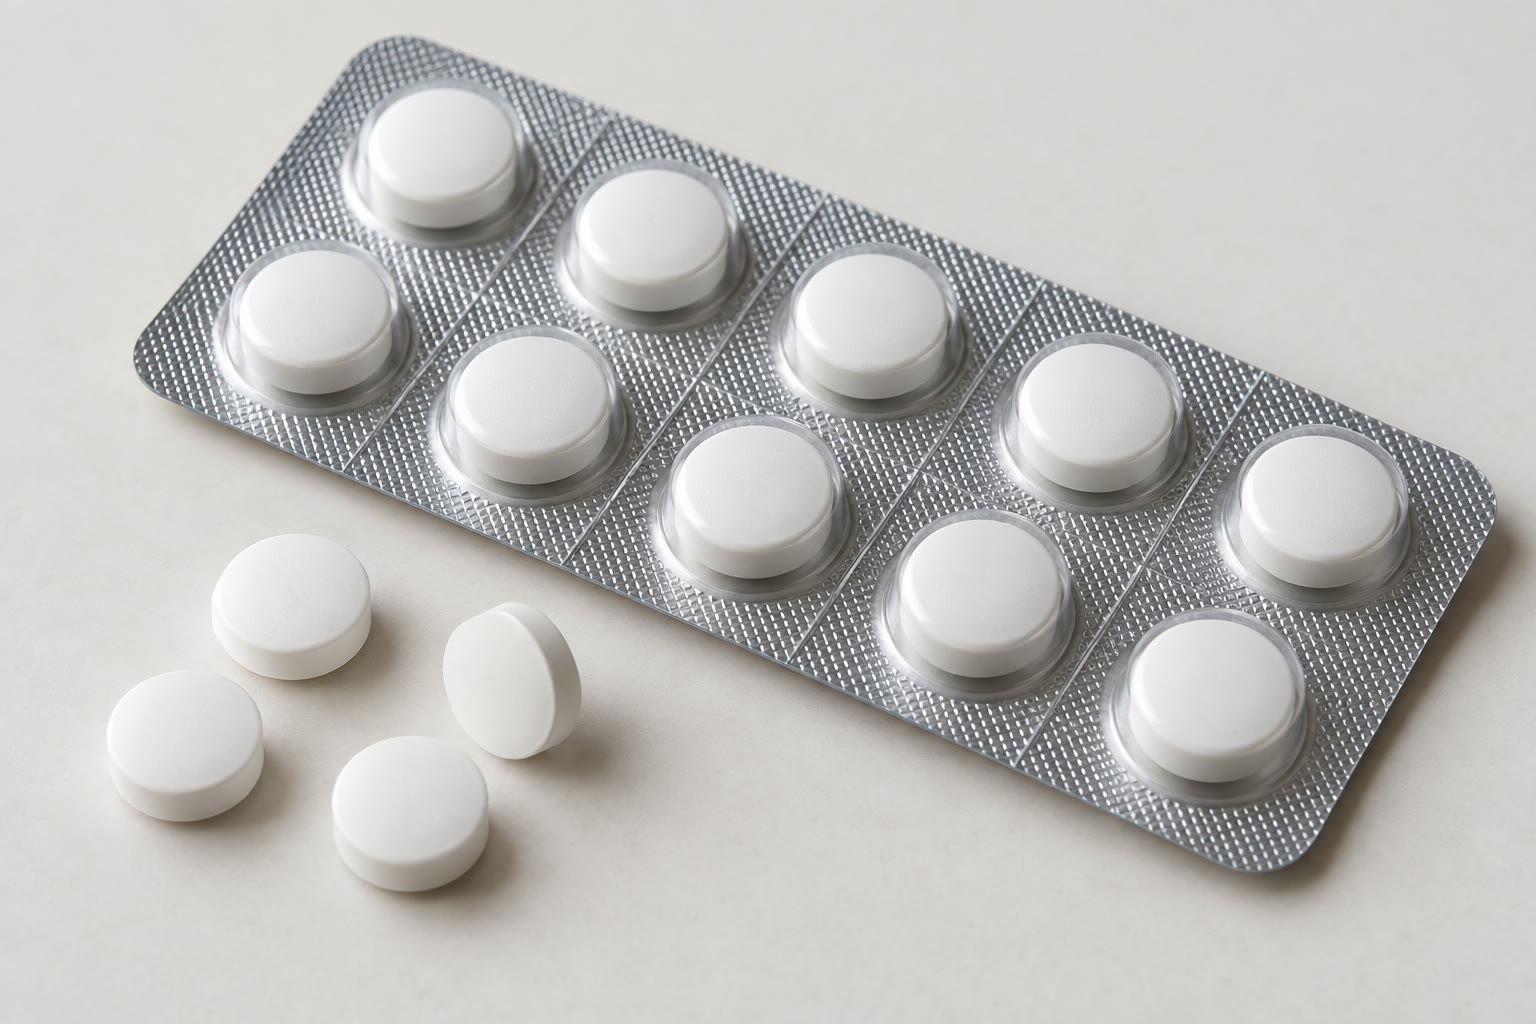
\includegraphics[width=0.45\linewidth]{images/book1/ai/g10-aspirin-tablets.jpg}

{\small Des comprimés d'aspirine~: chacun contient une masse pesée de la
substance pure, mélangée à un liant.}
\end{omfigure}

\section{Exercices}


\begin{exercise}[$\star$]\label{exo:g10:synthesis-yield:1}
Une \omterm{def:g10:synthesis-yield:synthesis}{synthèse} pourrait donner au plus \qty{5.0}{g} de produit~; on
obtient \qty{4.2}{g} de produit pur et sec. Calculer le \omterm{def:g10:synthesis-yield:yield}{rendement}.
\end{exercise}

\begin{exercise}[$\star$]\label{exo:g10:synthesis-yield:2}
Remettre dans l'ordre ces étapes d'une \omterm{def:g10:synthesis-yield:synthesis}{synthèse}~: mesure de la
température de fusion~; \omterm{def:g10:synthesis-yield:reflux}{chauffage à reflux}~; \omterm{def:g10:synthesis-yield:recrystallisation}{recristallisation}~;
\omterm{def:g10:synthesis-yield:vacuum-filtration}{filtration sous vide} du \omterm{def:g10:synthesis-yield:synthesis}{produit brut}~; pesée des \omterm{def:g7:chemical-reactions:reactant}{réactifs}.
\end{exercise}

\begin{exercise}[$\star$]\label{exo:g10:synthesis-yield:3}
Dans un montage à reflux, pourquoi l'eau de refroidissement entre-t-elle
dans le réfrigérant par le bas~? Pourquoi le haut du réfrigérant
reste-t-il ouvert~?
\end{exercise}

\begin{exercise}[$\star$]\label{exo:g10:synthesis-yield:4}
Quelles sont les deux propriétés que doit avoir un \omterm{def:g6:solutions-and-solubility:solute}{solvant} pour
recristalliser un produit~? Où finissent les impuretés~?
\end{exercise}

\begin{exercise}[$\star$]\label{exo:g10:synthesis-yield:5}
% ledger: mp:aspirin
Un échantillon d'aspirine synthétisée fond entre \qty{124}{\celsius} et
\qty{130}{\celsius}. L'aspirine pure fond vers \qty{135}{\celsius}.
L'échantillon est-il pur~? Que faut-il faire~?
\end{exercise}

\begin{exercise}[$\star\star$]\label{exo:g10:synthesis-yield:6}
\qty{2.00}{g} d'acide salicylique réagissent avec un excès d'anhydride
éthanoïque~; on obtient \qty{2.03}{g} d'aspirine pure et sèche. Calculer
la masse maximale d'aspirine et le \omterm{def:g10:synthesis-yield:yield}{rendement}.
\end{exercise}

\begin{exercise}[$\star\star$]\label{exo:g10:synthesis-yield:7}
Une élève pèse son aspirine encore humide et trouve un \omterm{def:g10:synthesis-yield:yield}{rendement} de
\qty{104}{\percent}. Expliquer. Peser le \omterm{def:g10:synthesis-yield:synthesis}{produit brut}, non purifié mais
sec, donnerait-il un \omterm{def:g10:synthesis-yield:yield}{rendement} trop élevé ou trop faible par rapport au
vrai \omterm{def:g10:synthesis-yield:yield}{rendement}~?
\end{exercise}

\begin{exercise}[$\star\star$]\label{exo:g10:synthesis-yield:8}
Donner deux avantages d'une \omterm{def:g10:synthesis-yield:vacuum-filtration}{filtration sous vide} sur une \omterm{def:g3:separating-mixtures:filter}{filtration}
ordinaire à travers un cône de papier, pour recueillir des cristaux.
\end{exercise}

\begin{exercise}[$\star\star$]\label{exo:g10:synthesis-yield:9}
Sur une plaque de chromatographie, le front du \omterm{def:g6:solutions-and-solubility:solute}{solvant} a parcouru
\qty{5.0}{cm}. La tache d'un produit synthétisé a parcouru
\qty{3.1}{cm}, celle de l'aspirine pure \qty{3.1}{cm}, celle de l'acide
salicylique \qty{2.2}{cm}. Calculer les trois rapports frontaux. Que
peut-on conclure au sujet du produit~?
\end{exercise}

\begin{exercise}[$\star\star$]\label{exo:g10:synthesis-yield:10}
La \omterm{def:g6:solutions-and-solubility:solubility}{solubilité} d'un produit dans deux \omterm{def:g6:solutions-and-solubility:solute}{solvants} est~:
\begin{center}
\begin{tabular}{lcc}
\hline
\omterm{def:g6:solutions-and-solubility:solute}{solvant} & à froid (\qty{20}{\celsius}) & à chaud (près de l'ébullition) \\
\hline
A & \qty{2}{g/L} & \qty{150}{g/L} \\
B & \qty{80}{g/L} & \qty{120}{g/L} \\
\hline
\end{tabular}
\end{center}
Quel \omterm{def:g6:solutions-and-solubility:solute}{solvant} convient le mieux pour une \omterm{def:g10:synthesis-yield:recrystallisation}{recristallisation}~? Pour
\qty{3.0}{g} de \omterm{def:g10:synthesis-yield:synthesis}{produit brut}, quel volume de \omterm{def:g6:solutions-and-solubility:solute}{solvant} chaud faut-il
environ, et quelle masse au plus reste dissoute une fois la solution
refroidie~?
\end{exercise}

\begin{exercise}[$\star\star$]\label{exo:g10:synthesis-yield:11}
Pourquoi le ballon d'un montage à reflux n'est-il jamais rempli à plus
de la moitié~? Pourquoi ajoute-t-on de la pierre ponce~?
\end{exercise}

\begin{exercise}[$\star\star\star$]\label{exo:g10:synthesis-yield:12}
Un médicament est fabriqué en deux étapes, de \omterm{def:g10:synthesis-yield:yield}{rendements}
\qty{80}{\percent} et \qty{70}{\percent}. Quel est le \omterm{def:g10:synthesis-yield:yield}{rendement} global~?
Que vaudrait-il pour trois étapes de \qty{90}{\percent} chacune~?
Pourquoi les chimistes cherchent-ils à fabriquer les médicaments en un
nombre d'étapes aussi faible que possible~?
\end{exercise}

\begin{exercise}[$\star\star\star$]\label{exo:g10:synthesis-yield:13}
% ledger: sol:aspirin-25
L'aspirine \omterm{def:g2:mixing-and-dissolving:dissolve}{se dissout} dans l'eau à raison d'environ \qty{3.3}{g/L} à
\qty{25}{\celsius}. On lave des cristaux avec \qty{50}{mL} d'eau à cette
température. Quelle masse d'aspirine peut-on perdre au plus~? Pourquoi
refroidit-on d'abord l'eau de lavage dans la glace~?
\end{exercise}

\begin{exercise}[$\star\star\star$]\label{exo:g10:synthesis-yield:14}
On \omterm{def:g6:pure-substances-and-mixtures:mixture}{mélange} \qty{2.76}{g} d'acide salicylique avec \qty{0.0500}{mol}
d'anhydride éthanoïque. Après la réaction, on ajoute de l'eau, qui
détruit l'excès d'anhydride~: \ce{C4H6O3 + H2O -> 2C2H4O2}.
\begin{enumerate}
  \item Remplir le \omterm{def:g10:reaction-progress-table:extent}{tableau d'avancement} de la \omterm{def:g10:synthesis-yield:synthesis}{synthèse}~; quelle quantité
        d'anhydride reste-t-il~?
  \item Quelle quantité totale d'acide éthanoïque est présente à la
        fin~?
\end{enumerate}
\end{exercise}

\begin{exercise}[$\star\star\star$]\label{exo:g10:synthesis-yield:15}
Une usine doit fabriquer \qty{1.00}{t} d'aspirine, avec un \omterm{def:g10:synthesis-yield:yield}{rendement}
global de \qty{85}{\percent} à partir de l'acide salicylique. Quelle
masse d'acide salicylique doit-elle acheter~?
\end{exercise}

\section{Problème~: fabriquer de l'aspirine}

\begin{problem}[{Problème du week-end --- de trois grammes d'acide
salicylique à un flacon d'aspirine pure~: quel est le rendement~?}]
\label{pb:g10:synthesis-yield:1}
% ledger: rho:acetic-anhydride, mp:aspirin, mp:salicylic, sol:aspirin-25, aw:C, aw:H, aw:O
Une classe fabrique de l'aspirine. Dans le ballon~: \qty{3.0}{g}
d'acide salicylique et \qty{6.0}{mL} d'anhydride éthanoïque, de masse
volumique \qty{1.08}{g/mL}, avec quelques gouttes d'acide~; le \omterm{def:g6:pure-substances-and-mixtures:mixture}{mélange}
est chauffé à reflux. Le \omterm{def:g10:synthesis-yield:synthesis}{produit brut} recueilli par \omterm{def:g10:synthesis-yield:vacuum-filtration}{filtration sous vide}
pèse \qty{3.6}{g} humide et \qty{3.3}{g} une fois sec. Après
\omterm{def:g10:synthesis-yield:recrystallisation}{recristallisation} et séchage, il reste \qty{2.7}{g} de cristaux blancs.

\medskip
\noindent\textbf{Partie I --- La réaction.}
\begin{enumerate}
  \item Vérifier que l'équation
        \ce{C7H6O3 + C4H6O3 -> C9H8O4 + C2H4O2} est ajustée.
  \item Calculer les \omterm{def:g10:the-mole:molar-mass}{masses molaires} de l'acide salicylique, de
        l'anhydride éthanoïque, de l'aspirine et de l'acide éthanoïque.
  \item Nommer les \omterm{def:g7:chemical-reactions:reactant}{réactifs}, le produit recherché et le sous-produit.
  \item Pourquoi chauffe-t-on le \omterm{def:g6:pure-substances-and-mixtures:mixture}{mélange} à reflux plutôt que dans un
        ballon ouvert~?
\end{enumerate}

\medskip
\noindent\textbf{Partie II --- La masse maximale.}
\begin{enumerate}[resume]
  \item Calculer la quantité initiale d'acide salicylique.
  \item Calculer la masse, puis la quantité, d'anhydride éthanoïque.
  \item Remplir le \omterm{def:g10:reaction-progress-table:extent}{tableau d'avancement}. Quel \omterm{def:g7:chemical-reactions:reactant}{réactif} est limitant~?
        Donner $x_{\max}$.
  \item En déduire la masse maximale d'aspirine.
  \item Pourquoi met-on en excès l'anhydride plutôt que l'acide
        salicylique~?
\end{enumerate}

\medskip
\noindent\textbf{Partie III --- Isoler et purifier.}
\begin{enumerate}[resume]
  \item Pourquoi ne peut-on pas utiliser la masse humide, \qty{3.6}{g},
        pour calculer un \omterm{def:g10:synthesis-yield:yield}{rendement}~?
  \item Calculer le \omterm{def:g10:synthesis-yield:yield}{rendement} en \omterm{def:g10:synthesis-yield:synthesis}{produit brut} sec.
  \item Pourquoi la \omterm{def:g10:synthesis-yield:recrystallisation}{recristallisation} diminue-t-elle la masse~?
  \item Les cristaux ont été lavés avec \qty{30}{mL} d'eau à
        \qty{25}{\celsius}, température à laquelle l'aspirine \omterm{def:g2:mixing-and-dissolving:dissolve}{se dissout}
        à raison d'environ \qty{3.3}{g/L}. Quelle masse a pu être perdue
        au plus de cette façon~?
  \item Calculer le \omterm{def:g10:synthesis-yield:yield}{rendement} en produit pur.
\end{enumerate}

\medskip
\noindent\textbf{Partie IV --- Contrôler le produit.}
\begin{enumerate}[resume]
  \item Les cristaux recristallisés fondent nettement à
        \qty{135}{\celsius}. Que montre ce résultat~?
  \item Le \omterm{def:g10:synthesis-yield:synthesis}{produit brut} fondait entre \qty{120}{\celsius} et
        \qty{131}{\celsius}. Que montre ce résultat~?
  \item Sur une plaque de chromatographie, le \omterm{def:g10:synthesis-yield:synthesis}{produit brut} donne deux
        taches, l'une à la hauteur de l'aspirine pure et l'autre à la
        hauteur de l'acide salicylique~; le produit recristallisé donne
        une seule tache, à la hauteur de l'aspirine. Conclure.
  \item La tache du produit recristallisé a parcouru \qty{3.1}{cm} et le
        front du \omterm{def:g6:solutions-and-solubility:solute}{solvant} \qty{5.0}{cm}. Calculer son \omterm{def:g10:chemical-species:retention-factor}{rapport frontal}.
  \item De la transformation et de la \omterm{def:g10:synthesis-yield:recrystallisation}{recristallisation}, quelle partie
        du travail a fait perdre le plus d'aspirine~?
  \item Donner la réponse finale~: quel est le \omterm{def:g10:synthesis-yield:yield}{rendement} de la
        \omterm{def:g10:synthesis-yield:synthesis}{synthèse}~?
\end{enumerate}
\end{problem}
